
\section{Thuật toán điều khiển}

Hệ thống tự động dựa trên luồng di chuyển của sản phẩm được chia thành năm quá trình chính như Hình~\ref{c3:workflow}:

\begin{figure}
    \centering
    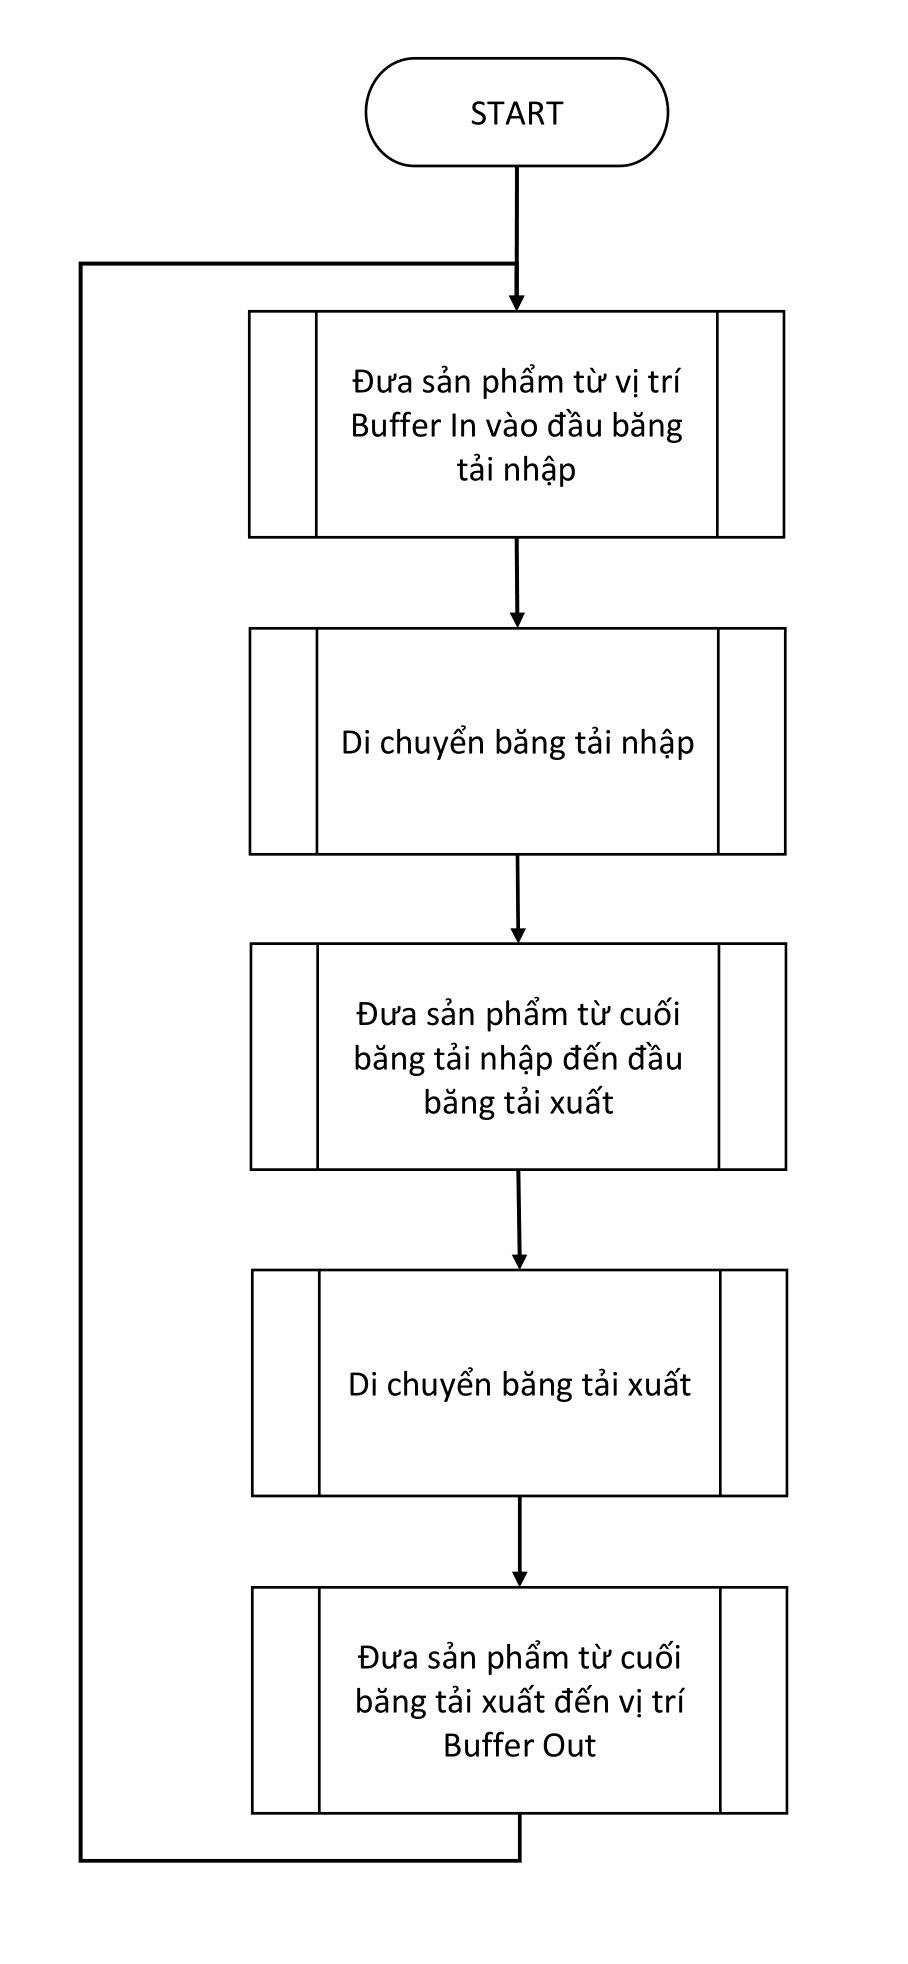
\includegraphics[width=0.68\textwidth]{figures/Chapter3/workflow.png}
    \caption{Quy trình tổng quát}
    \label{c3:workflow}
\end{figure}

\begin{enumerate}
    \item Đưa sản phẩm từ vị trí Buffer In vào đầu băng tải nhập bằng robot Hyundai.
    \item Di chuyển băng tải nhập đưa sản phẩm từ đầu băng tải đến vị trí chụp ảnh; sau khi chụp ảnh, băng tải tiếp tục di chuyển sản phẩm đến cuối băng tải.
    \item Đưa sản phẩm từ cuối băng tải nhập đến đầu băng tải xuất bằng robot Yaskawa.
    \item Di chuyển băng tải xuất từ đầu băng tải đến cuối băng tải.
    \item Đưa sản phẩm từ cuối băng tải xuất đến vị trí Buffer Out bằng robot Hyundai.
\end{enumerate}

Việc phân tách hệ thống thành các quá trình riêng biệt giúp dễ dàng xây dựng lưu trình điều khiển chi tiết, đồng thời đơn giản hóa quá trình lập trình và kiểm soát hoạt động của toàn hệ thống.
%=================================
\newpage
\subsection{Quá trình 1: Đưa sản phẩm từ Buffer In vào đầu băng tải nhập}

\begin{figure}[h]
    \centering
    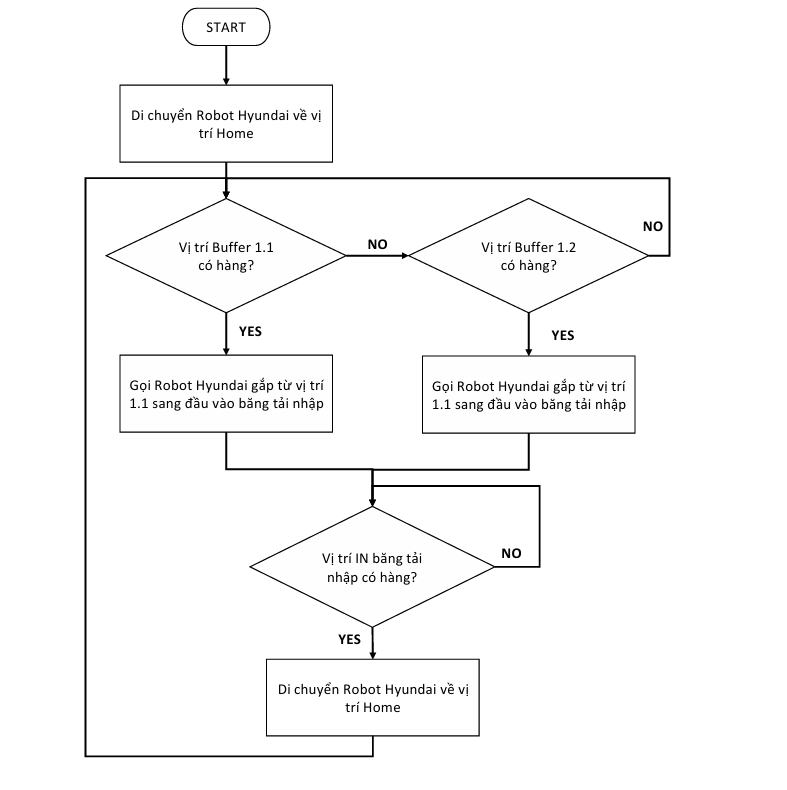
\includegraphics[width=1\textwidth]{figures/Chapter3/workflow1.png}
    \caption{Quá trình 1.}
    \label{c3:workflow1}
\end{figure}
%=================================================
\newpage
\subsection{Quá trình 2: Di chuyển băng tải nhập}

\begin{figure}[h]
    \centering
    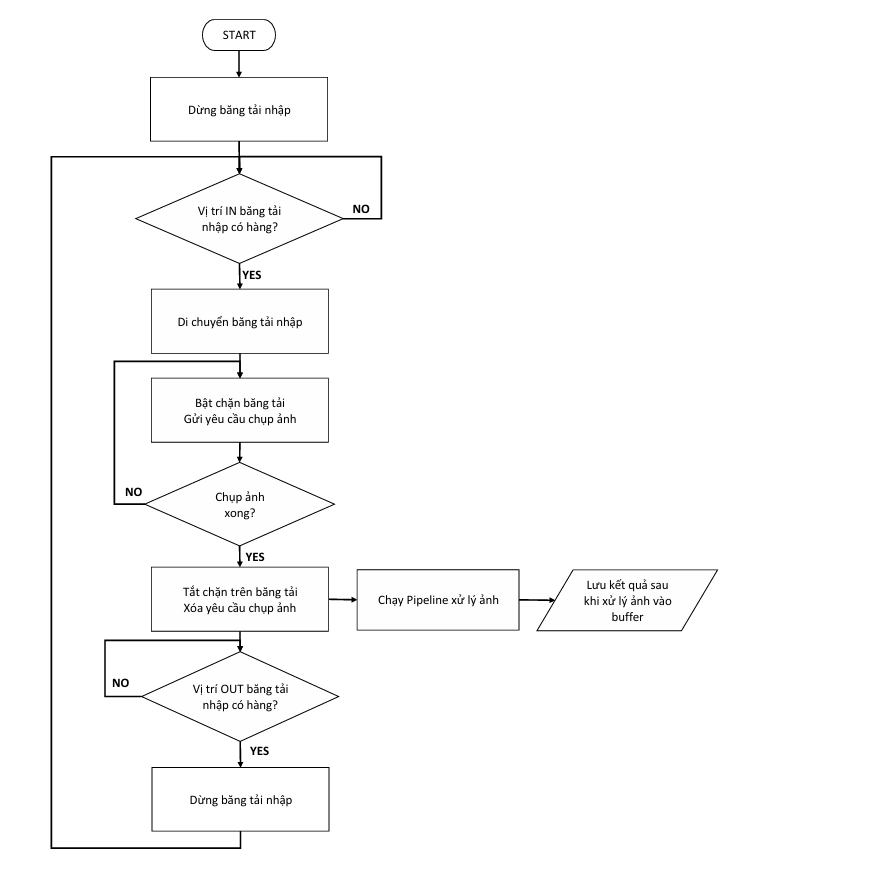
\includegraphics[width=1\textwidth]{figures/Chapter3/workflow2.png}
    \caption{Quá trình 2.}
    \label{c3:workflow2}
\end{figure}
%=================================================
\newpage
\subsection{Quá trình 3: Đưa sản phẩm từ băng tải nhập vào băng tải xuất}

\begin{figure}[h]
    \centering
    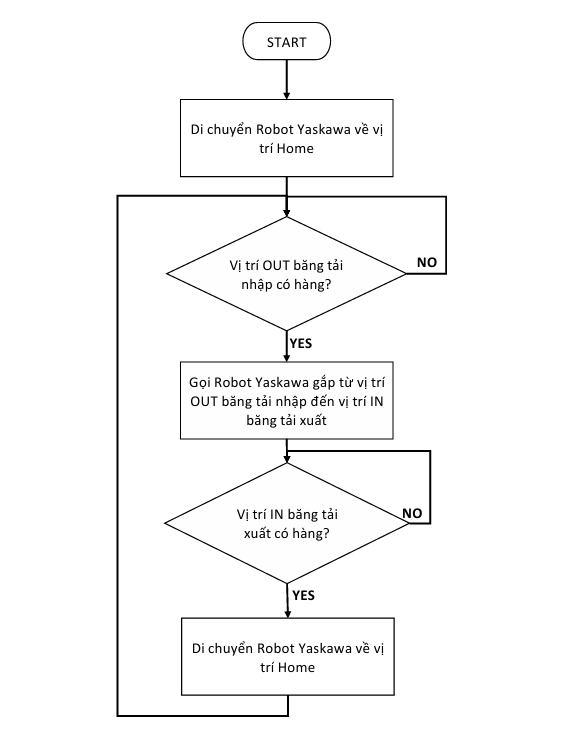
\includegraphics[width=0.8\textwidth]{figures/Chapter3/workflow3.png}
    \caption{Quá trình 3.}
    \label{c3:workflow3}
\end{figure}
%=================================================
\newpage
\subsection{Quá trình 4: Di chuyển băng tải xuất}

\begin{figure}[h]
    \centering
    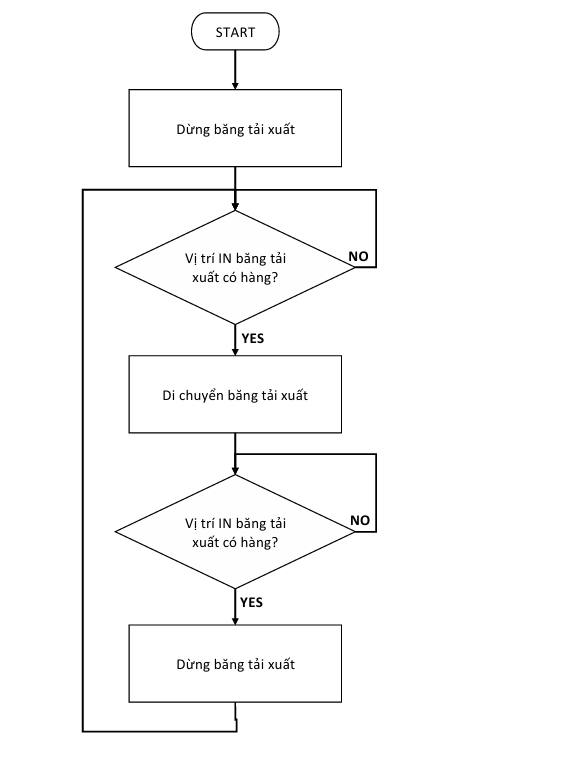
\includegraphics[width=0.8\textwidth]{figures/Chapter3/workflow4.png}
    \caption{Quá trình 4.}
    \label{c3:workflow4}
\end{figure}
%======================================================
\newpage
\subsection{Quá trình 5: Đưa sản phẩm từ băng tải xuất đến Buffer Out}

\begin{figure}[h]
    \centering
    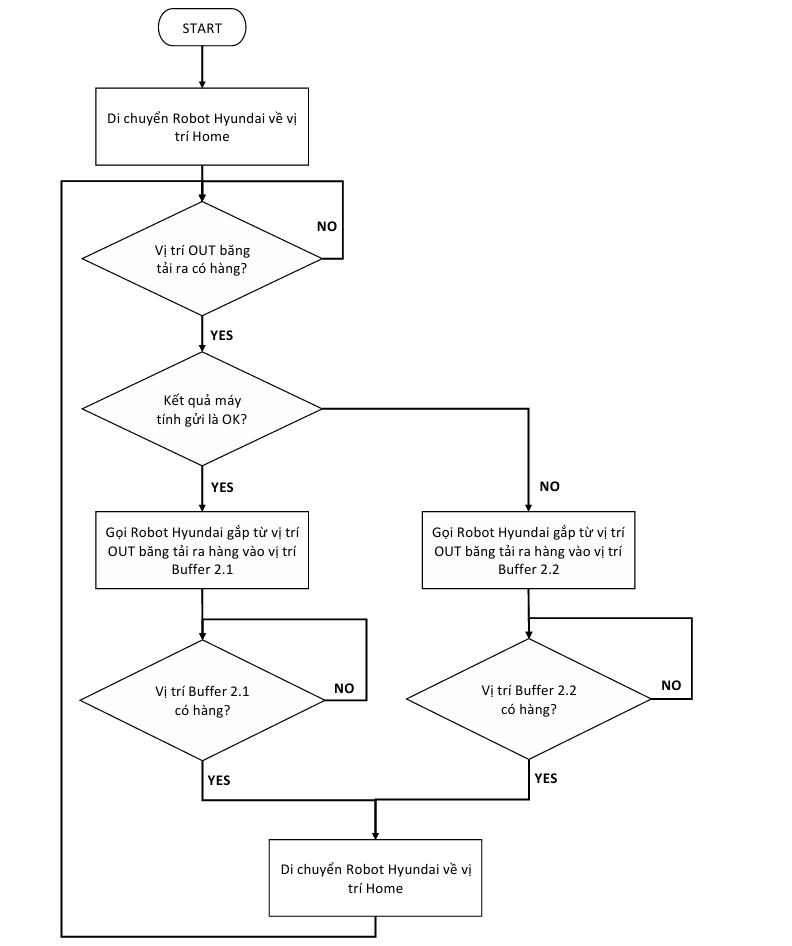
\includegraphics[width=0.8\textwidth]{figures/Chapter3/workflow5.png}
    \caption{Quá trình 5.}
    \label{c3:workflow5}
\end{figure}


% =======================
% PHẦN 3: CẤU HÌNH HỆ THỐNG
% =======================
\newpage

